\chapter{Cấu tạo và nguyên lý hoạt động}

\section{Cơ sở lý thuyết}
Hệ thống điều khiển xe robot không dây sử dụng cảm biến MPU6050 \cite{mpu6050-datasheet} và băm xung PWM trên vi điều khiển STM32F103C8T6 \cite{noviello2022mastering} được phát triển dựa trên nguyên lý của lý thuyết điều khiển thời gian thực và truyền thông không dây tầm ngắn. 

Về cơ bản, hệ thống được chia làm hai khối độc lập tương tác với nhau thông qua mạng truyền thông không dây:
\begin{itemize}
    \item \textbf{Khối phát (Transmitter / Thiết bị điều khiển cầm tay):} Đảm nhiệm vai trò thu thập thông tin về trạng thái chuyển động quán tính của tay người dùng. Cảm biến MPU6050 tích hợp gia tốc kế (Accelerometer) và con quay hồi chuyển (Gyroscope) sẽ liên tục đo đạc gia tốc hướng trục và vận tốc góc trong không gian ba chiều \cite{mpu6050-datasheet}. Vi điều khiển STM32F103C8T6 (dựa trên nhân ARM Cortex-M3 \cite{yiu2013definitive}) đóng vai trò xử lý trung tâm khối phát, đọc các dữ liệu thô này qua giao tiếp I2C \cite{stm32-hal}, áp dụng các công thức lượng giác để tính toán ra hai góc nghiêng đặc trưng là góc Pitch (nghiêng trước/sau) và góc Roll (nghiêng trái/phải). Các góc này sau đó được ánh xạ sang các lệnh điều khiển hướng (tiến, lùi, rẽ trái, rẽ phải) và đóng gói thành chuỗi dữ liệu gửi đi qua module Bluetooth HC-05 hoạt động ở chế độ Master thông qua cổng giao tiếp nối tiếp UART.
    \item \textbf{Khối thu (Receiver / Xe robot):} Tiếp nhận dữ liệu không dây qua module Bluetooth HC-05 hoạt động ở chế độ Slave (giao tiếp nối tiếp UART với vi điều khiển). Bộ vi điều khiển STM32F103C8T6 ở khối thu thực hiện giải mã gói tin nhận được, xác định lệnh di chuyển và tính toán tốc độ tương ứng. Tốc độ động cơ được kiểm soát bằng cách thay đổi hệ số chu kỳ (duty cycle) của xung điều chế độ rộng xung (PWM) cấp cho các chân điều tốc của driver cầu H TB6612FNG. Đồng thời, hướng quay của các động cơ DC chổi than được quyết định bởi mức logic (HIGH/LOW) xuất ra các chân GPIO điều hướng kết nối với driver.
\end{itemize}

\begin{figure}[H]
    \centering
    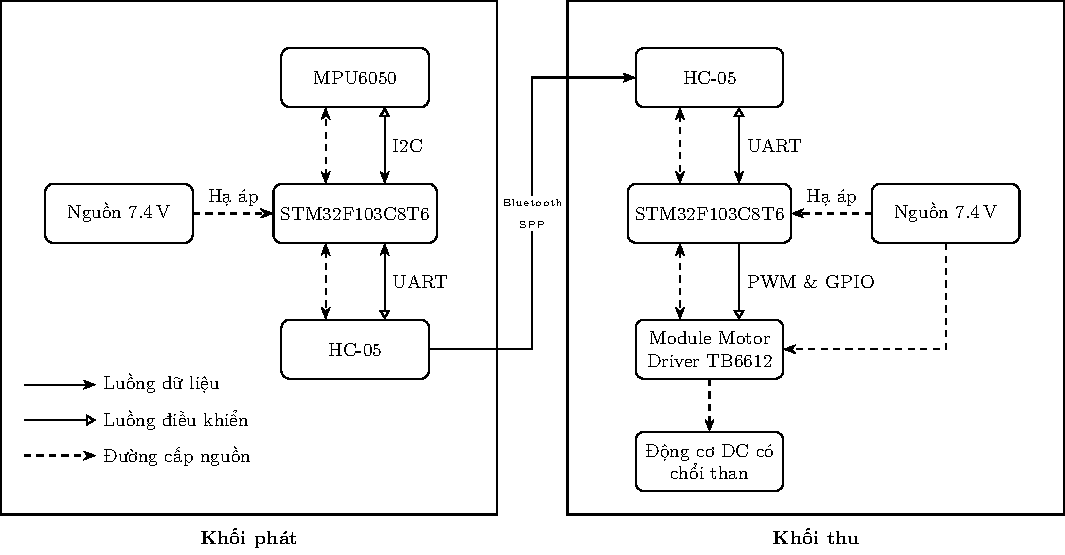
\includegraphics[width=0.95\textwidth]{tikz/architecture.pdf}
    \caption{Sơ đồ kiến trúc phần cứng và luồng tương tác trong hệ thống}
    \label{fig:architecture}
\end{figure}

\section{Thiết lập bảng FRDPARRC}
Bảng FRDPARRC (Functional Requirements - Design Parameters - Analysis - Reference - Risk - Countermeasure) là công cụ quan trọng trong thiết kế kỹ thuật hệ thống, giúp ánh xạ các yêu cầu chức năng thành các thông số thiết kế cụ thể, đồng thời phân tích rủi ro và đề xuất các giải pháp khắc phục tương ứng để đảm bảo độ tin cậy của hệ thống.

Dưới đây là bảng FRDPARRC được thiết lập cho dự án:

\begin{table}[H]
\centering
\renewcommand{\arraystretch}{1.3}
\caption{Bảng FRDPARRC của hệ thống}
\label{tab:frdparrc}
\changefontsizes{9pt}
\begin{tabularx}{0.98\textwidth}{|c|>{\raggedright\arraybackslash}X|>{\raggedright\arraybackslash}p{2.1cm}|>{\raggedright\arraybackslash}p{2.1cm}|>{\raggedright\arraybackslash}p{1.8cm}|>{\raggedright\arraybackslash}p{2.1cm}|>{\raggedright\arraybackslash}p{2.3cm}|}
\hline
\multicolumn{1}{|c|}{\textbf{STT}} & \multicolumn{1}{c|}{\textbf{FR}} & \multicolumn{1}{c|}{\textbf{DP}} & \multicolumn{1}{c|}{\textbf{A}} & \multicolumn{1}{c|}{\textbf{R}} & \multicolumn{1}{c|}{\textbf{R}} & \multicolumn{1}{c|}{\textbf{C}} \\
\hline
1 & Đo quán tính và góc nghiêng của tay cầm & Cảm biến quán tính MPU6050 (giao tiếp I2C) & Đọc gia tốc thô, tính góc Pitch, Roll bằng hàm lượng giác & Datasheet MPU6050 \cite{mpu6050-datasheet} & Nhiễu rung từ tay người và trôi sai số con quay hồi chuyển & Thiết lập vùng chết (deadzone), hiệu chuẩn offset lúc khởi động \\
\hline
2 & Xử lý trung tâm khối phát (tay cầm) & Vi điều khiển STM32\-F103 (lõi Cortex-M3) & Tính toán góc và đóng gói dữ liệu lệnh gửi qua UART & Ref. Manual STM32F103 \cite{stm32-hal} & Sụt áp nguồn phát gây treo hoặc reset vi điều khiển & Sử dụng ổn áp AMS1117-3.3V và thêm tụ lọc nguồn 10uF gần chân VDD \\
\hline
3 & Giao tiếp không dây nối tiếp & Module Bluetooth HC-05 (Master-Slave) & Truyền nhận gói dữ liệu điều khiển qua UART (Baud 9600) & Datasheet HC-05 & Nhiễu sóng 2.4GHz và mất kết nối khi vượt khoảng cách cho phép & Cài đặt tính năng dừng an toàn (fail-safe) tự ngắt động cơ khi mất kết nối \\
\hline
4 & Xử lý trung tâm và điều khiển khối thu & Vi điều khiển STM32\-F103 (khối thu) & Giải mã gói tin UART, xử lý logic lái và xuất tín hiệu điều khiển & Ref. Manual STM32F103 \cite{stm32-hal} & Nhiễu điện từ động cơ gây treo chip hoặc sai lệch tín hiệu điều khiển & Sử dụng Watchdog Timer, tối ưu bộ đệm UART và lắp tụ chống nhiễu \\
\hline
5 & Điều khiển công suất động cơ DC & Driver cầu H TB6612FNG và động cơ DC chổi than & Cấp xung PWM điều tốc (Timer 2) và xuất GPIO điều khiển chiều & Datasheet TB6612 & Dòng khởi động lớn gây sụt áp nguồn chính hoặc quá dòng khi kẹt động cơ & Tách nguồn động cơ và vi xử lý, thêm tụ điện 470uF lọc nguồn \\
\hline
6 & Cung cấp nguồn năng lượng ổn định & Pin Li-ion \qty{7.4}{\volt} cho xe, pin \qty{3.7}{\volt} cho tay cầm & Đo điện áp ngõ ra của bộ ổn áp dưới tải nặng & Datasheet LM2596 / AMS1117 & Quá nhiệt hoặc sụt áp khi hoạt động dưới tải nặng & Sử dụng module hạ áp Buck LM2596 và ổn áp AMS1117 hiệu suất cao \\
\hline
\end{tabularx}
\end{table}

\section{Nghiên cứu}
Quá trình nghiên cứu và phát triển hệ thống được nhóm thực hiện tuần tự qua các giai đoạn nghiên cứu lý thuyết, lựa chọn linh kiện, thiết kế phần cứng và lập trình phần mềm:
\begin{itemize}
    \item \textbf{Nghiên cứu nguyên lý cảm biến và xử lý số liệu:} Tìm hiểu cấu trúc thanh ghi của cảm biến MPU6050 \cite{mpu6050-register}, nguyên lý đo gia tốc quán tính để tính toán góc nghiêng dựa trên vectơ trọng lực của Trái Đất. Nhóm đã nghiên cứu các công thức lượng giác (\texttt{atan2f}) \cite{serway2018physics} để chuyển đổi gia tốc thô trên các trục X, Y, Z thành góc Pitch và Roll. Nhóm cũng tìm hiểu hiện tượng nhiễu rung động học và trôi sai số tích lũy để thiết lập thuật toán hiệu chuẩn offset lúc khởi động và cài đặt dải chết (deadzone) hợp lý nhằm triệt tiêu dao động nhỏ khi tay cầm đứng yên.
    \item \textbf{Nghiên cứu tài nguyên vi điều khiển:} Tìm hiểu tập lệnh HAL (Hardware Abstraction Layer) của STM32 \cite{stm32-hal} để cấu hình các ngoại vi phần cứng: giao tiếp I2C1 tốc độ \qty{100}{\kilo\hertz} đọc cảm biến \cite{noviello2022mastering}, USART1 tốc độ BaudRate \qty{9600}{bps} truyền thông nối tiếp, và Timer 2 cấu hình các kênh xuất xung PWM tần số \qty{\approx1}{\kilo\hertz} để điều khiển động cơ DC di chuyển êm ái, tránh phát ra tiếng rít từ cuộn dây động cơ.
    \item \textbf{Nghiên cứu giao tiếp truyền thông không dây:} Tìm hiểu cơ chế ghép nối tự động Master-Slave giữa hai module Bluetooth HC-05 sử dụng tập lệnh cấu hình AT thông qua cổng nối tiếp. Thiết lập liên kết không dây ổn định dưới dạng truyền nhận nối tiếp trong suốt, bảo đảm dữ liệu gửi đi từ khối phát được phản hồi tức thời tại khối thu.
    \item \textbf{Nghiên cứu mạch động lực điều khiển:} Phân tích đặc tính dòng điện và điện áp hoạt động của động cơ DC chổi than dưới tải thực tế \cite{alexander2021fundamentals}. Nghiên cứu mạch cầu H TB6612FNG, nhận thấy ưu điểm vượt trội của nó so với dòng mạch cũ L298N nhờ sử dụng công nghệ cầu H MOSFET giúp giảm sụt áp nội bộ và tỏa ít nhiệt hơn, bảo vệ tốt nguồn pin của xe.
\end{itemize}

\section{Cấu tạo của hệ thống điều khiển xe robot không dây}
Hệ thống hoàn chỉnh được cấu thành từ các thành phần linh kiện phần cứng phối hợp chặt chẽ với nhau, chia làm hai khối chức năng riêng biệt:

\subsection{Khối phát (Thiết bị điều khiển cầm tay)}
\begin{itemize}
    \item \textbf{Vi điều khiển STM32F103C8T6:} Thực hiện khởi tạo hệ thống, đọc dữ liệu cảm biến MPU6050 qua bus I2C, tính toán góc nghiêng và gửi gói tin điều khiển qua UART.
    \item \textbf{Cảm biến quán tính MPU6050:} Đo gia tốc và vận tốc góc 3 trục, kết nối với STM32 qua giao tiếp I2C1 (chân SCL - PB6, SDA - PB7).
    \item \textbf{Module Bluetooth HC-05 (Master):} Truyền nối tiếp không dây dữ liệu từ chân TXD của USART1 (PA9) trên STM32 sang khối thu.
    \item \textbf{Khối nguồn khối phát:} Sử dụng pin sạc Li-ion \qty{3.7}{\volt} kết hợp mạch sạc và mạch ổn áp AMS1117-\qty{3.3}{\volt} cấp nguồn ổn định cho vi điều khiển và cảm biến.
\end{itemize}

\subsection{Khối thu (Xe robot)}
\begin{itemize}
    \item \textbf{Vi điều khiển STM32F103C8T6:} Tiếp nhận dữ liệu từ module Bluetooth qua USART1 (chân RX - PA10), xử lý logic điều hướng và xuất các tín hiệu PWM điều tốc cùng GPIO điều khiển hướng động cơ.
    \item \textbf{Module Bluetooth HC-05 (Slave):} Nhận tín hiệu sóng vô tuyến Bluetooth từ khối phát, truyền dữ liệu nối tiếp vào chân RX (PA10) của vi điều khiển.
    \item \textbf{Driver cầu H TB6612FNG:} Nhận 2 kênh xung PWM (PA0, PA1) và các chân điều hướng GPIO (PA2, PA3, PA4, PA5) để điều khiển tốc độ và chiều quay của các động cơ DC.
    \item \textbf{Động cơ DC chổi than:} 4 động cơ DC kèm hộp số giảm tốc và bánh xe cao su để tạo lực kéo cho xe.
    \item \textbf{Khối nguồn khối thu:} Sử dụng pack pin Li-ion \qty{7.4}{\volt} cấp nguồn trực tiếp cho driver TB6612\-FNG chạy động cơ. Module hạ áp Buck LM2596 được sử dụng để hạ áp xuống \qty{5}{\volt} (và tiếp tục ổn áp xuống \qty{3.3}{\volt} thông qua mạch AMS1117) cấp nguồn cho vi điều khiển và module Blue\-tooth, đảm bảo hệ thống hoạt động ổn định và chống nhiễu sụt áp khi động cơ vận hành.
\end{itemize}

\subsection{Sơ đồ nguyên lý của khối thu}
Hình \ref{fig:receiver} mô tả bản vẽ sơ đồ nguyên lý thiết kế mạch chi tiết cho khối thu, mô tả đầy đủ các đường đi dây, kết nối cổng UART, I2C, xung điều tốc PWM và phân bổ các nhánh cấp nguồn điện:

\begin{figure}
    \centering
    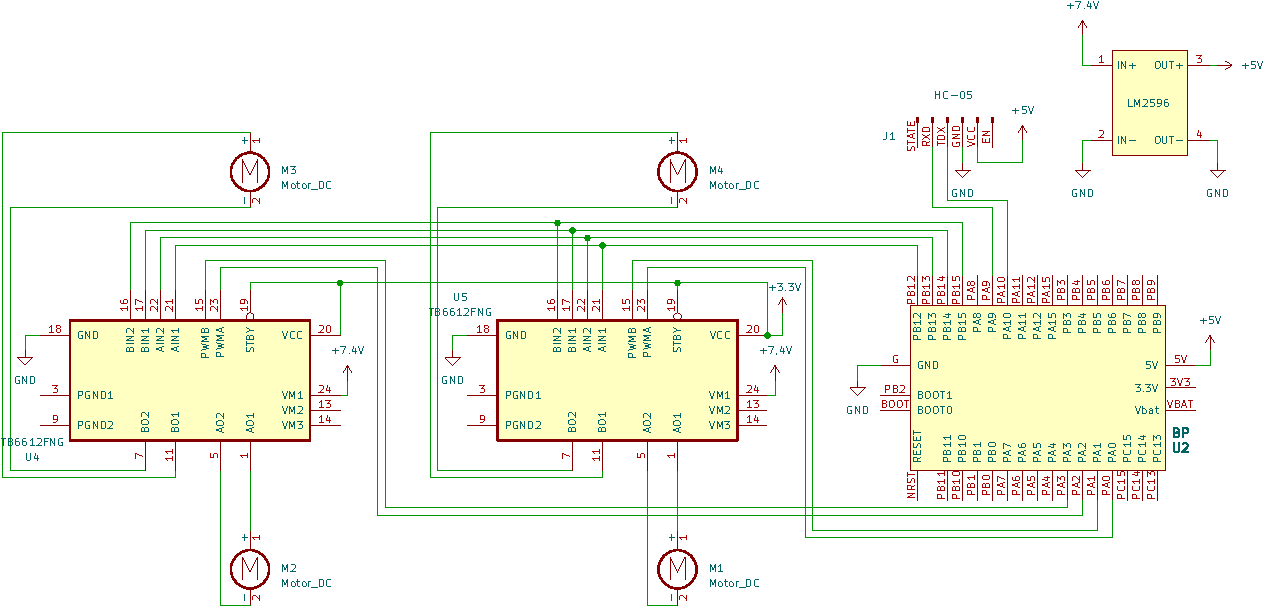
\includegraphics[angle=90, height=0.9\textheight]{Schematic/Schematic-Receiver.pdf}
    \caption{Sơ đồ nguyên lý khối thu}
    \label{fig:receiver}
\end{figure}

\section{Sơ đồ nguyên lý của khối phát}
Hình {\ref{fig:transmitter}} mô tả bản vẽ sơ đồ nguyên lý thiết kế mạch chi tiết của khối phát:

\begin{figure}[p]
    \centering
    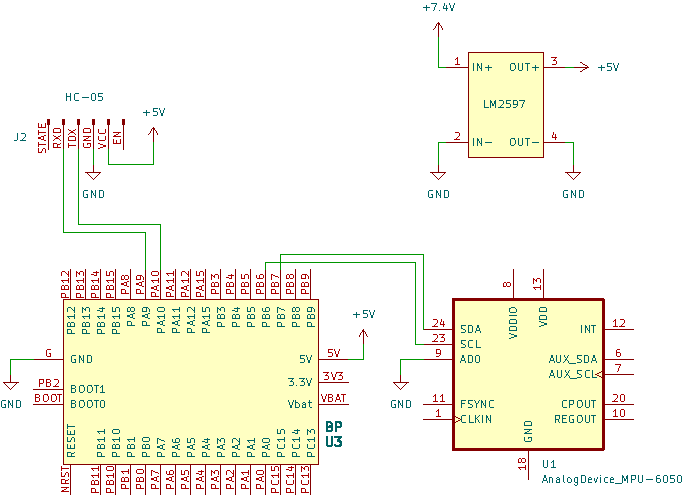
\includegraphics[angle=90, width=0.72\textwidth]{Schematic/Schematic-Transmitter.pdf}
    \caption{Sơ đồ nguyên lý khối phát}
    % \input{Schematic/Schematic-Transmitter.pdf_tex}
    \label{fig:transmitter}
\end{figure}

\section{Nguyên lý hoạt động và Giải thuật điều khiển}
Hệ thống điều khiển hoạt động dựa trên sự phối hợp chặt chẽ giữa khối phát và khối thu. Nguyên lý vận hành chi tiết và các thuật toán điều khiển được mô tả cụ thể dưới đây.

\subsection{Nguyên lý hoạt động toàn hệ thống}
Quy trình vận hành khép kín của hệ thống diễn ra liên tục theo chu kỳ thời gian thực:
\begin{enumerate}
    \item \textbf{Khối phát}: Vi điều khiển STM32 đọc dữ liệu gia tốc 3 trục từ cảm biến MPU6050 qua giao tiếp I2C. Dựa trên dữ liệu gia tốc này, thuật toán lượng giác tính toán góc nghiêng Pitch ($\theta$) và Roll ($\phi$) của bàn tay:
    \[ \theta = \mathrm{atan2}(A_x, \sqrt{A_y^2 + A_z^2}) \times \frac{180}{\pi} \]
    \[ \phi = \mathrm{atan2}(A_y, \sqrt{A_x^2 + A_z^2}) \times \frac{180}{\pi} \]
    Sau khi áp dụng bộ lọc dải chết (Deadzone) để loại bỏ rung lắc tay nhẹ, STM32 phân loại góc nghiêng thành các lệnh di chuyển tương ứng và gửi gói tin qua UART đến module Bluetooth HC-05 (Master).
    \item \textbf{Khối thu}: Module Bluetooth HC-05 (Slave) nhận sóng RF và chuyển tiếp gói dữ liệu đến STM32 khối thu qua UART. Vi điều khiển giải mã gói tin, kiểm tra tính hợp lệ và cập nhật trạng thái hoạt động của xe. Đồng thời, một cơ chế kiểm tra thời gian chờ (Timeout) liên tục giám sát trạng thái kết nối. Nếu quá 0.3 giây (300 ms) không nhận được gói tin mới, hệ thống tự động kích hoạt chế độ Fail-safe để bảo vệ an toàn cho xe.
\end{enumerate}

\subsection{Lưu đồ giải thuật hệ thống}
Giải thuật lập trình cho vi xử lý ở cả hai khối được xây dựng nhằm tối ưu hóa tính thời gian thực và độ an toàn của xe robot di động.

\subsubsection{Giải thuật khối phát}
Thuật toán khối phát hoạt động theo mô hình vòng lặp vô hạn (Infinite Loop):
\begin{itemize}
    \item Khởi tạo hệ thống: Thiết lập GPIO, cấu hình giao tiếp I2C1 và USART1, cấu hình dải đo gia tốc cho MPU6050.
    \item Đọc dữ liệu cảm biến: Đọc 6 byte dữ liệu gia tốc hướng trục từ MPU6050.
    \item Tính toán góc nghiêng: Áp dụng công thức hàm lượng giác để xác định góc Pitch và Roll.
    \item Xử lý dải chết (Deadzone): Nếu góc nghiêng nhỏ hơn $8^\circ$, coi như tay nằm ngang (Lệnh Dừng). Nếu vượt quá $8^\circ$, hệ thống bắt đầu tính toán giá trị điều khiển và ánh xạ góc nghiêng sang mức tốc độ PWM tương ứng theo hàm phi tuyến.
    \item Truyền dữ liệu: Đóng gói ký tự điều khiển (tiến, lùi, trái, phải, dừng) và gửi ra cổng USART1.
    \item Trì hoãn (Delay): Chờ \qty{50}{\milli\second} trước khi lặp lại chu kỳ mới.
\end{itemize}

\subsubsection{Giải thuật khối thu}
Thuật toán khối thu hoạt động kết hợp giữa ngắt nhận dữ liệu UART và vòng lặp chính:
\begin{itemize}
    \item Khởi tạo hệ thống: Thiết lập các chân điều hướng động cơ (GPIO Output), cấu hình bộ định thời Timer 2 phát xung PWM điều tốc, cấu hình ngắt nhận dữ liệu UART (USART1).
    \item Vòng lặp chính:
    \begin{itemize}
        \item Liên tục kiểm tra biến đếm thời gian (Timeout Counter). Nếu thời gian trôi qua từ lần nhận gói tin cuối cùng vượt quá \qty{300}{\milli\second}, hệ thống tự động đưa xe về trạng thái dừng khẩn cấp (Fail-Safe), tắt xung PWM và ngắt dòng động cơ.
        \item Khi nhận được ký tự điều khiển hợp lệ qua ngắt UART: Cập nhật lệnh di chuyển, đặt lại biến đếm thời gian về 0, điều chỉnh các chân GPIO hướng quay và thay đổi chu kỳ nhiệm vụ (Duty Cycle) của xung PWM để thay đổi tốc độ động cơ theo yêu cầu điều tốc.
    \end{itemize}
\end{itemize}

\begin{figure}
    \centering
    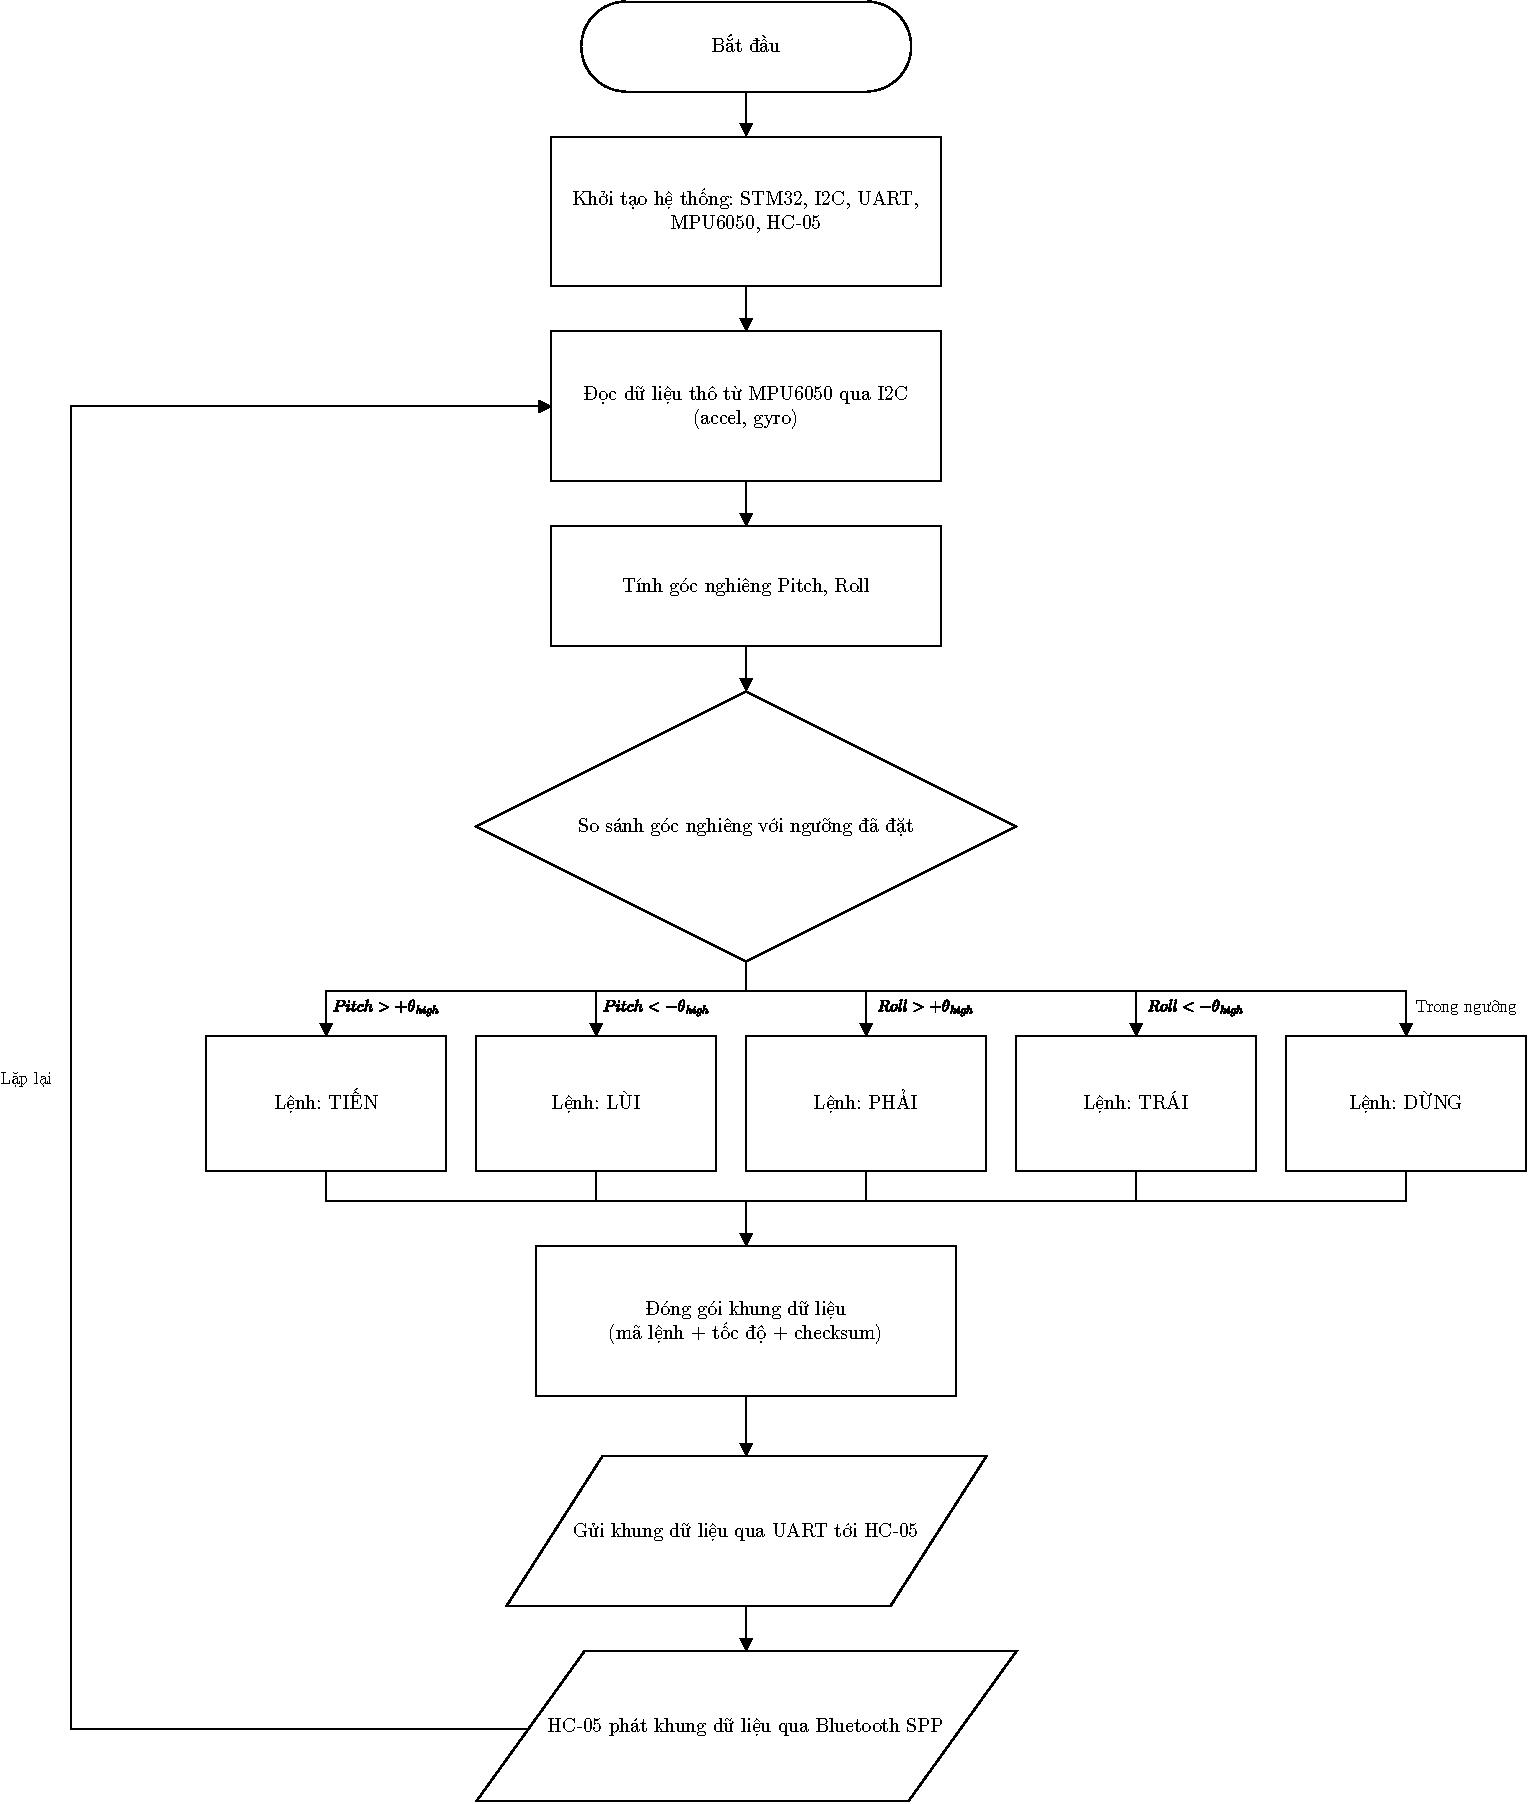
\includegraphics[width=\textwidth]{Drawio/Transmitter_Flowchart.drawio.pdf}
    \caption{Lưu đồ giải thuật chi tiết của khối phát}
    \label{fig:transmitter-flowchart}
\end{figure}

\begin{figure}
    \centering
    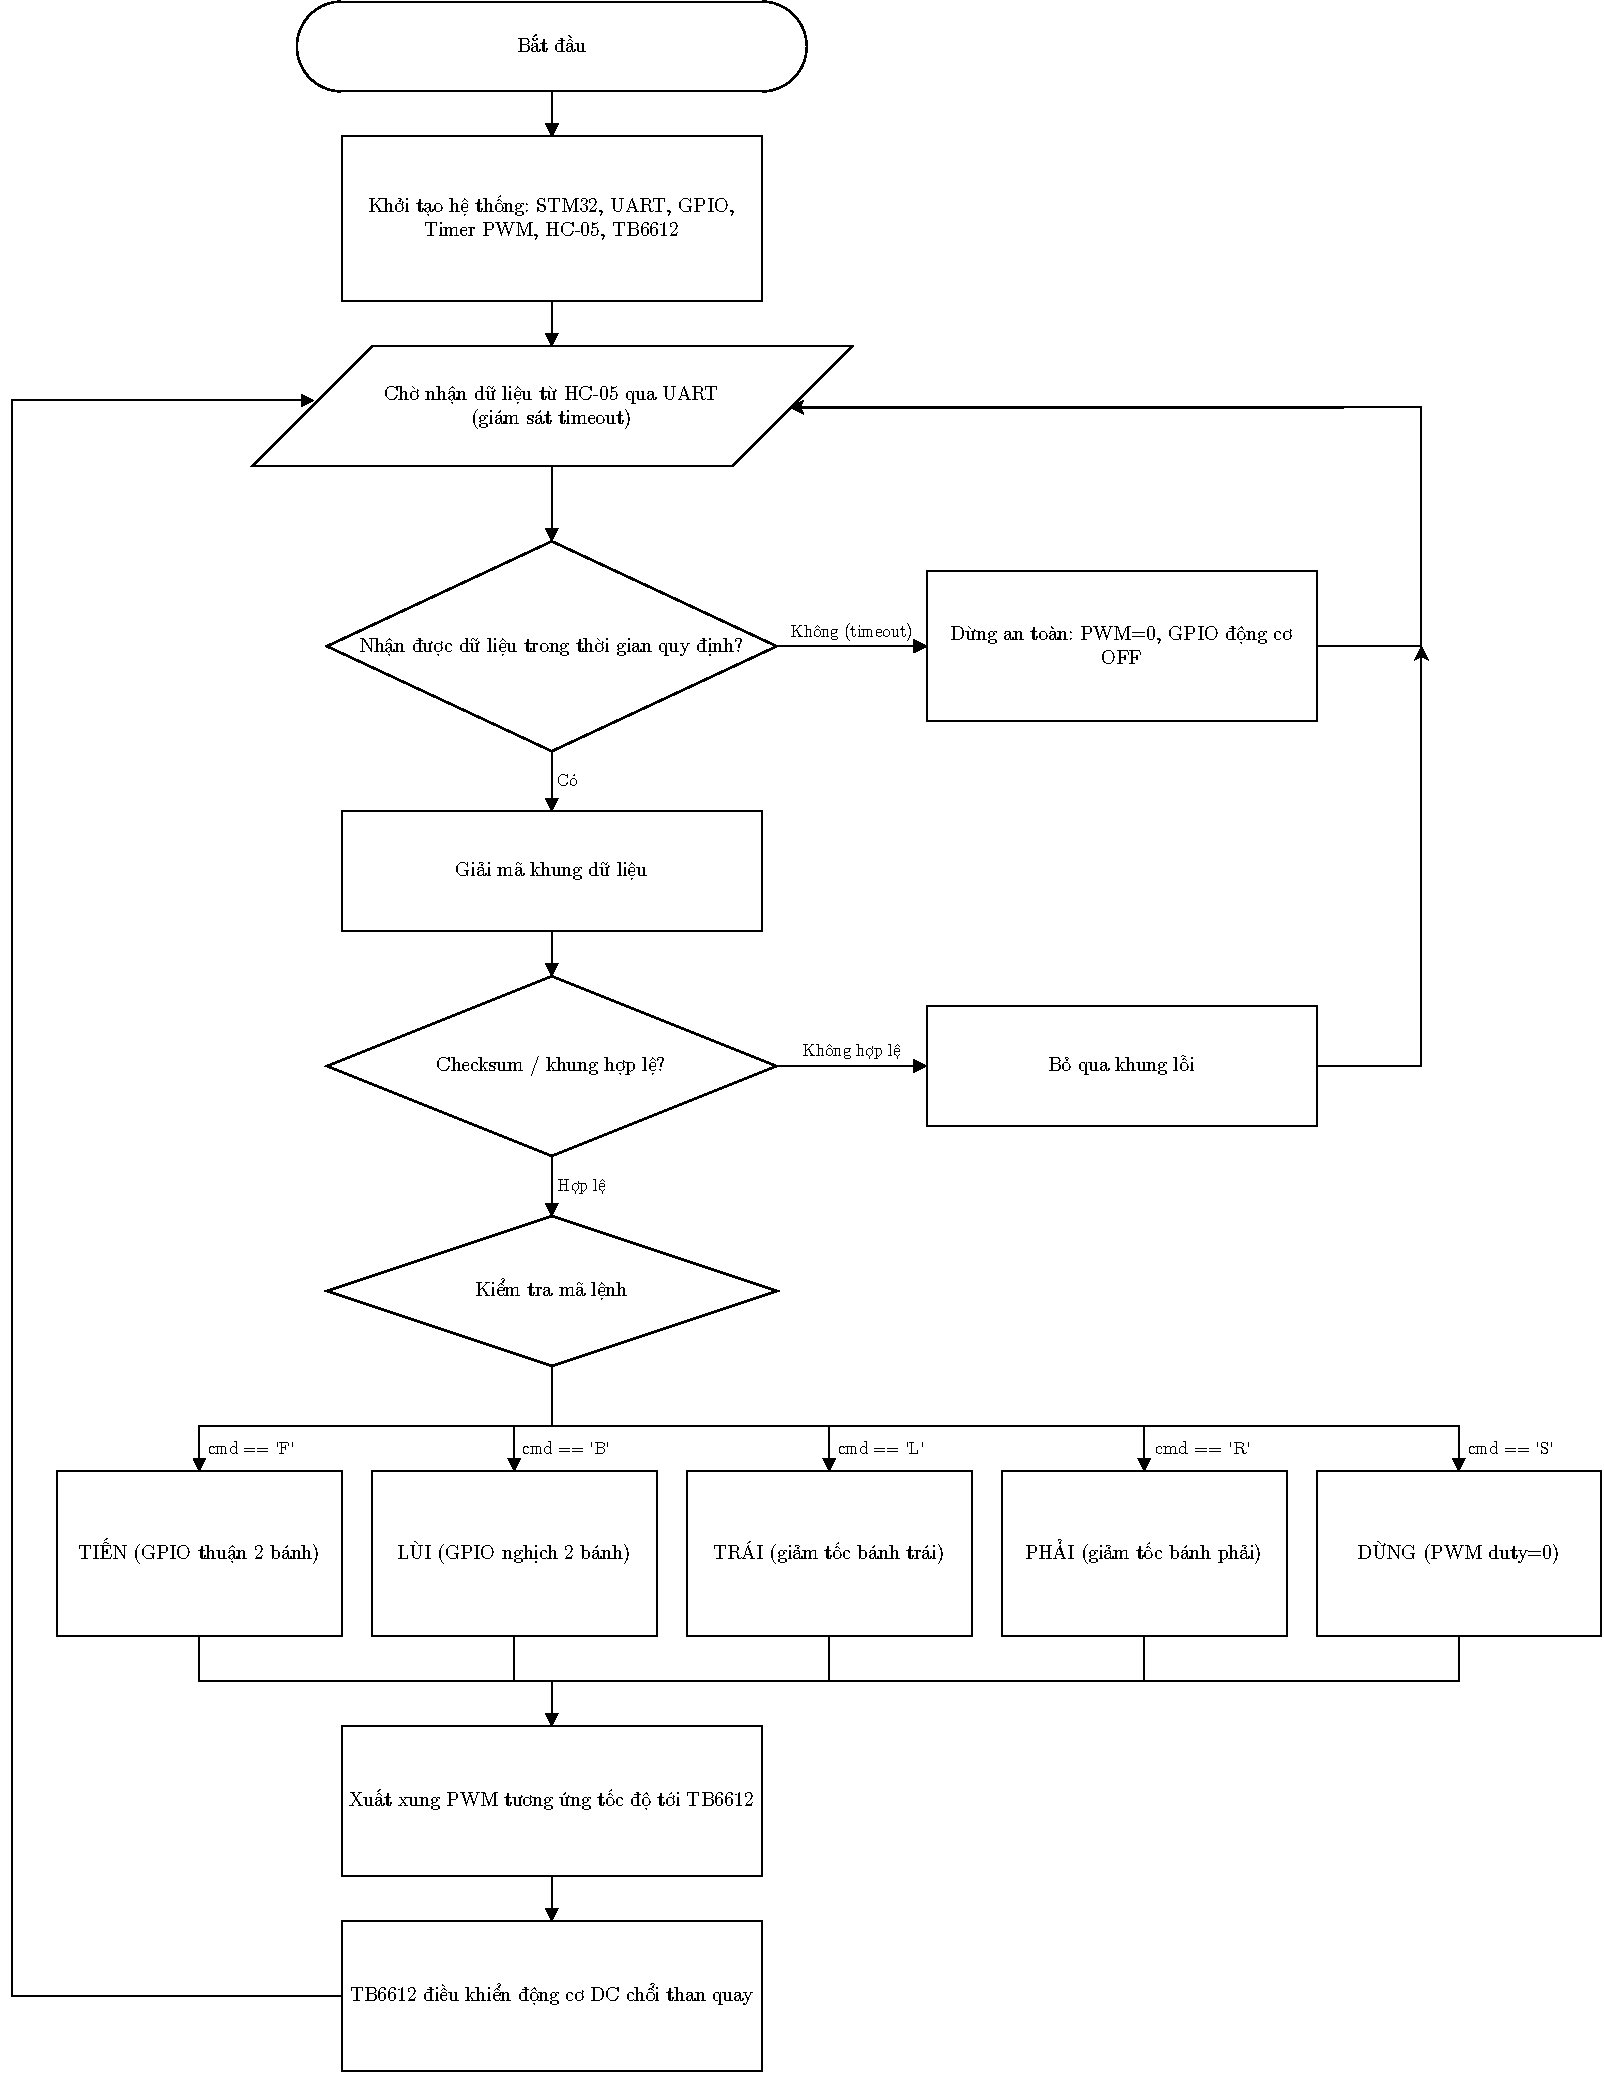
\includegraphics[width=\textwidth]{Drawio/Receiver_Flowchart.drawio.pdf}
    \caption{Lưu đồ giải thuật chi tiết của khối thu}
    \label{fig:receiver-flowchart}
\end{figure}

\subsection{Máy trạng thái finite (FSM) của hệ thống}
Để quản lý hành vi chuyển động và đảm bảo tính an toàn cao nhất, giải thuật điều khiển khối thu được thiết kế dưới dạng một máy trạng thái finite (Finite State Machine). Các trạng thái hoạt động chính của xe robot bao gồm:
\begin{enumerate}
    \item \textbf{STATE\_STOP (Trạng thái dừng):} Trạng thái mặc định khi khởi động xe hoặc khi góc nghiêng tay nằm trong dải chết. PWM ngắt (0\%), các chân điều hướng động cơ ở mức logic thấp.
    \item \textbf{STATE\_FORWARD (Trạng thái tiến):} Xe di chuyển về phía trước. Kích hoạt khi góc Pitch tay cầm hướng lên phía trước vượt ngưỡng. Tốc độ xe tỷ lệ thuận với góc nghiêng.
    \item \textbf{STATE\_BACKWARD (Trạng thái lùi):} Xe di chuyển lùi về sau. Kích hoạt khi góc Pitch hướng về phía sau vượt ngưỡng.
    \item \textbf{STATE\_LEFT (Trạng thái rẽ trái):} Xe rẽ trái bằng cách quay ngược chiều giữa hai bên bánh xe hoặc giảm tốc độ bên trái, tăng tốc độ bên phải. Kích hoạt khi góc Roll nghiêng sang trái.
    \item \textbf{STATE\_RIGHT (Trạng thái rẽ phải):} Xe rẽ phải bằng cách giảm tốc độ bên phải, tăng tốc độ bên trái. Kích hoạt khi góc Roll nghiêng sang phải.
    \item \textbf{STATE\_FAIL\_SAFE (Trạng thái dừng an toàn):} Trạng thái khẩn cấp kích hoạt ngay lập tức khi mất tín hiệu kết nối Bluetooth giữa khối phát và khối thu quá thời gian quy định (0.3 giây hoặc 300 ms). Trạng thái này có độ ưu tiên cao nhất, lập tức khóa đầu ra động cơ và chỉ cho phép chuyển sang trạng thái \textbf{STATE\_STOP} khi kết nối Bluetooth được thiết lập lại thành công.
\end{enumerate}

Dưới đây là bảng chuyển đổi trạng thái của hệ thống điều khiển:

\begin{table}[H]
\centering
\renewcommand{\arraystretch}{1.3}
\caption{Bảng chuyển đổi trạng thái (FSM) của khối thu}
\label{tab:fsm_transitions}
\changefontsizes{9pt}
\begin{tabularx}{0.98\textwidth}{|>{\raggedright\arraybackslash}p{3.3cm}|>{\raggedright\arraybackslash}p{3.3cm}|>{\raggedright\arraybackslash}X|>{\raggedright\arraybackslash}p{3.2cm}|}
\hline
\textbf{Trạng thái hiện tại} & \textbf{Trạng thái tiếp theo} & \textbf{Điều kiện chuyển trạng thái} & \textbf{Hành động thực hiện} \\
\hline
Mọi trạng thái & STATE\_FAIL\_SAFE & Mất kết nối Bluetooth quá 0.3 giây (300 ms) & Tắt PWM (0\%), dừng khẩn cấp xe \\
\hline
STATE\_FAIL\_SAFE & STATE\_STOP & Kết nối Bluetooth được khôi phục & Reset bộ đệm, chờ lệnh mới \\
\hline
STATE\_STOP & STATE\_FORWARD & Góc Pitch tay cầm $> 8^\circ$ & Xuất GPIO tiến, phát PWM điều tốc \\
\hline
STATE\_STOP & STATE\_BACKWARD & Góc Pitch tay cầm $< -8^\circ$ & Xuất GPIO lùi, phát PWM điều tốc \\
\hline
STATE\_STOP & STATE\_LEFT & Góc Roll tay cầm $< -8^\circ$ & Xuất GPIO rẽ trái, phát PWM điều tốc \\
\hline
STATE\_STOP & STATE\_RIGHT & Góc Roll tay cầm $> 8^\circ$ & Xuất GPIO rẽ phải, phát PWM điều tốc \\
\hline
STATE\_FORWARD / BACKWARD / LEFT / RIGHT & STATE\_STOP & Góc Pitch và Roll nằm trong dải chết ($\pm 8^\circ$) & Tắt xung PWM, dừng động cơ xe \\
\hline
\end{tabularx}
\end{table}

\begin{figure}
    \centering
    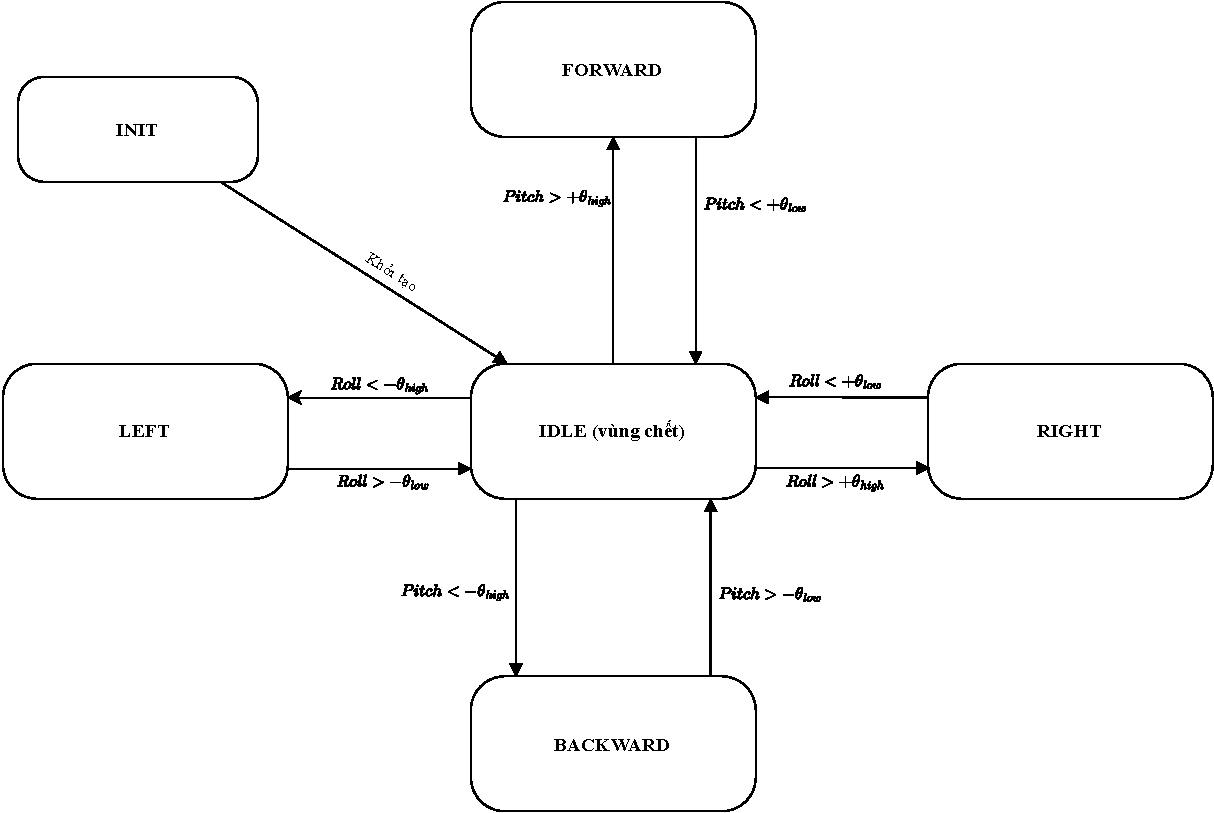
\includegraphics[width=\textwidth]{Drawio/Transmitter_FSP.drawio.pdf}
    \caption{Sơ đồ máy trạng thái khối phát}
    \label{fig:receiver-fsm}
\end{figure}

\begin{figure}
    \centering
    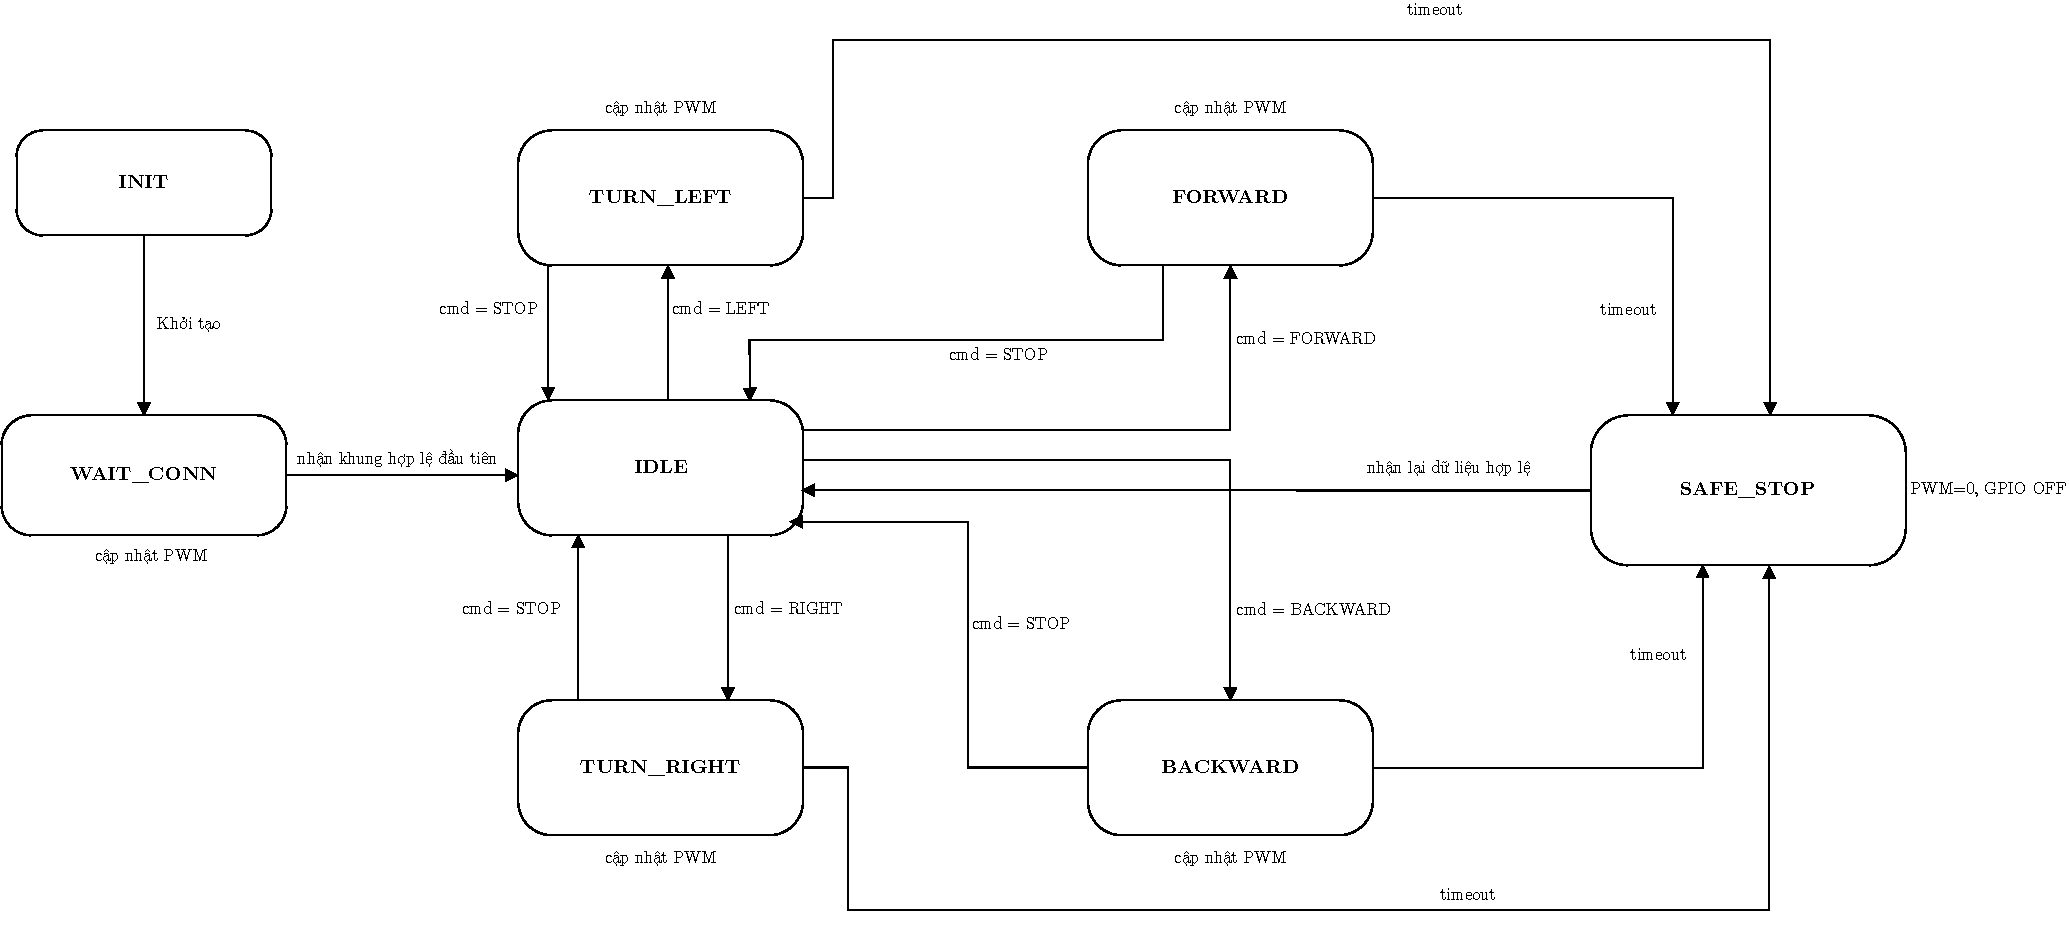
\includegraphics[width=\textwidth]{Drawio/Receiver_FSP.drawio.pdf}
    \caption{Sơ đồ máy trạng thái khối thu}
    \label{fig:transmitter-fsm}
\end{figure}